\documentclass[10pt, compress]{beamer}

\usetheme{glasgow}

\usepackage{booktabs}
\usepackage[scale=2]{ccicons}
\usepackage{minted}
\usepackage{bookmark}
\usepgfplotslibrary{dateplot}

\usemintedstyle{trac}

% ($ (A)!r!(B) $) the location of images to be used
\graphicspath{{src/}}

%% Customisation
% \newcommand{\V}[1]{\v} % vectors \v{c}
% \renewcommand{\v}[1]{\mathbf{#1}} % vectors
\newcommand{\ti}[1]{\tilde{#1}} % spectral representation
\newcommand{\tnsr}[1]{\underline{\underline{#1}}}

% Symbols
\renewcommand{\O}{\omega}  % omega
\newcommand{\E}{\varepsilon}  % epsilon
\renewcommand{\u}{\mu}  % mu
\newcommand{\p}{\rho}  % rho
\newcommand{\x}{\times}  % times
\renewcommand{\inf}{\infty}  % infinity
\newcommand{\infint}{\int\limits_{-\inf}^\inf} % integral by R
\newcommand{\e}{\mathrm{e}} % Straight-up exponential
\renewcommand{\j}{{j}\mkern1mu} % Straight-up exponential
\newcommand{\iu}{\mathrm{i}\mkern1mu}

\newcommand\ddfrac[2]{\frac{\displaystyle #1}{\displaystyle #2}}

\title{High Frequency Communication Systems}
\subtitle{Lecture 3}
\date{Spring 2021}
\author{Hasan T Abbas \& Qammer H Abbasi}
% \institute{}

\begin{document}

\maketitle

%%%%%%%%%%%%%%%%%%%%%%%%%%%%%%%%%%%%%%%%%%
%%%%%%%%%%%%%%%%%%%%%%%%%%%%%%%%%%%%%%%%%%
%%%%%%%%%%%%%%%%%%%%%%%%%%%%%%%%%%%%%%%%%%
\begin{frame}[fragile]
  \frametitle{Lecture Outline}
  \begin{outline}[itemize]
    \1 Antennas and Radiation
    \1 Potential Functions
    \1 Antenna Characteristics
  \end{outline}
\end{frame}
%%%%%%%%%%%%%%%%%%%%%%%%%%%%%%%%%%%%%%%%%%
%%%%%%%%%%%%%%%%%%%%%%%%%%%%%%%%%%%%%%%%%%
%%%%%%%%%%%%%%%%%%%%%%%%%%%%%%%%%%%%%%%%%%
\begin{frame}[fragile]
  \frametitle{Sources of Electromagnetic Fields}
  \begin{outline}
    \1 A distribution of currents and charges can generate and \color{red}{radiate} electromagnetic fields
    \2 The distribution is typically localised in a region of space
    \2 As an example, a simple wire can act as an \textit{antenna}
    \1 We are interested in determining the electromagnetic fields in space, given a current distribution
  \end{outline}
\end{frame}

\begin{frame}
  \frametitle{Antenna}
  \begin{columns}[T] % align columns
    \begin{column}{.4\textwidth}
      \begin{outline}
        \1 Antennas are most widely used for wireless communications
        \1 Modern antenna invention is attributed to Heinrich Hertz (1887)
        \2 Radio system was developed by Guglielmo Marconi (1897)
        \1 Due to the \textit{duality} principle, an antenna can also act as a receiver to EM radiation
      \end{outline}
    \end{column}
    \begin{column}[T]{.6\textwidth}
      \begin{figure}
        \centering
        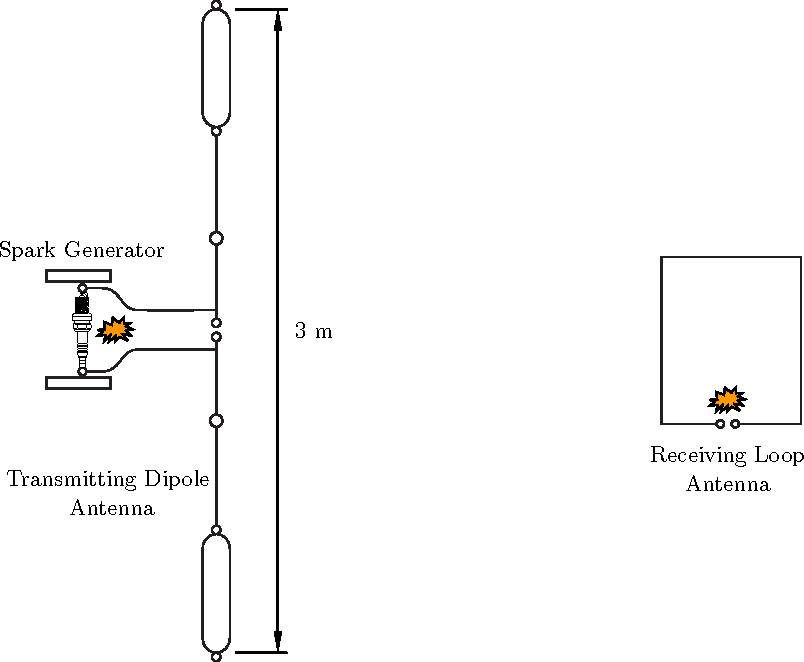
\includegraphics[width=.9\textwidth]{antenna_hertz.pdf}
        \caption{The Hertz's invention}
      \end{figure}
    \end{column}%
  \end{columns}
\end{frame}

\begin{frame}
  \frametitle{How Antennas Radiate}
  \begin{columns}[T] % align columns
    \begin{column}{.4\textwidth}
      \begin{outline}
        \1 We need a \color{red}{disturbance} in the EM fields
        \2 Most commonly, this is caused by a time-varying electric current
        \1 The disturbance also depends on the nature of the antenna
        \2 For a wire antenna, the discontinuities at the ends cause radiation
      \end{outline}
    \end{column}
    \begin{column}[T]{.6\textwidth}
      \begin{figure}
        \centering
        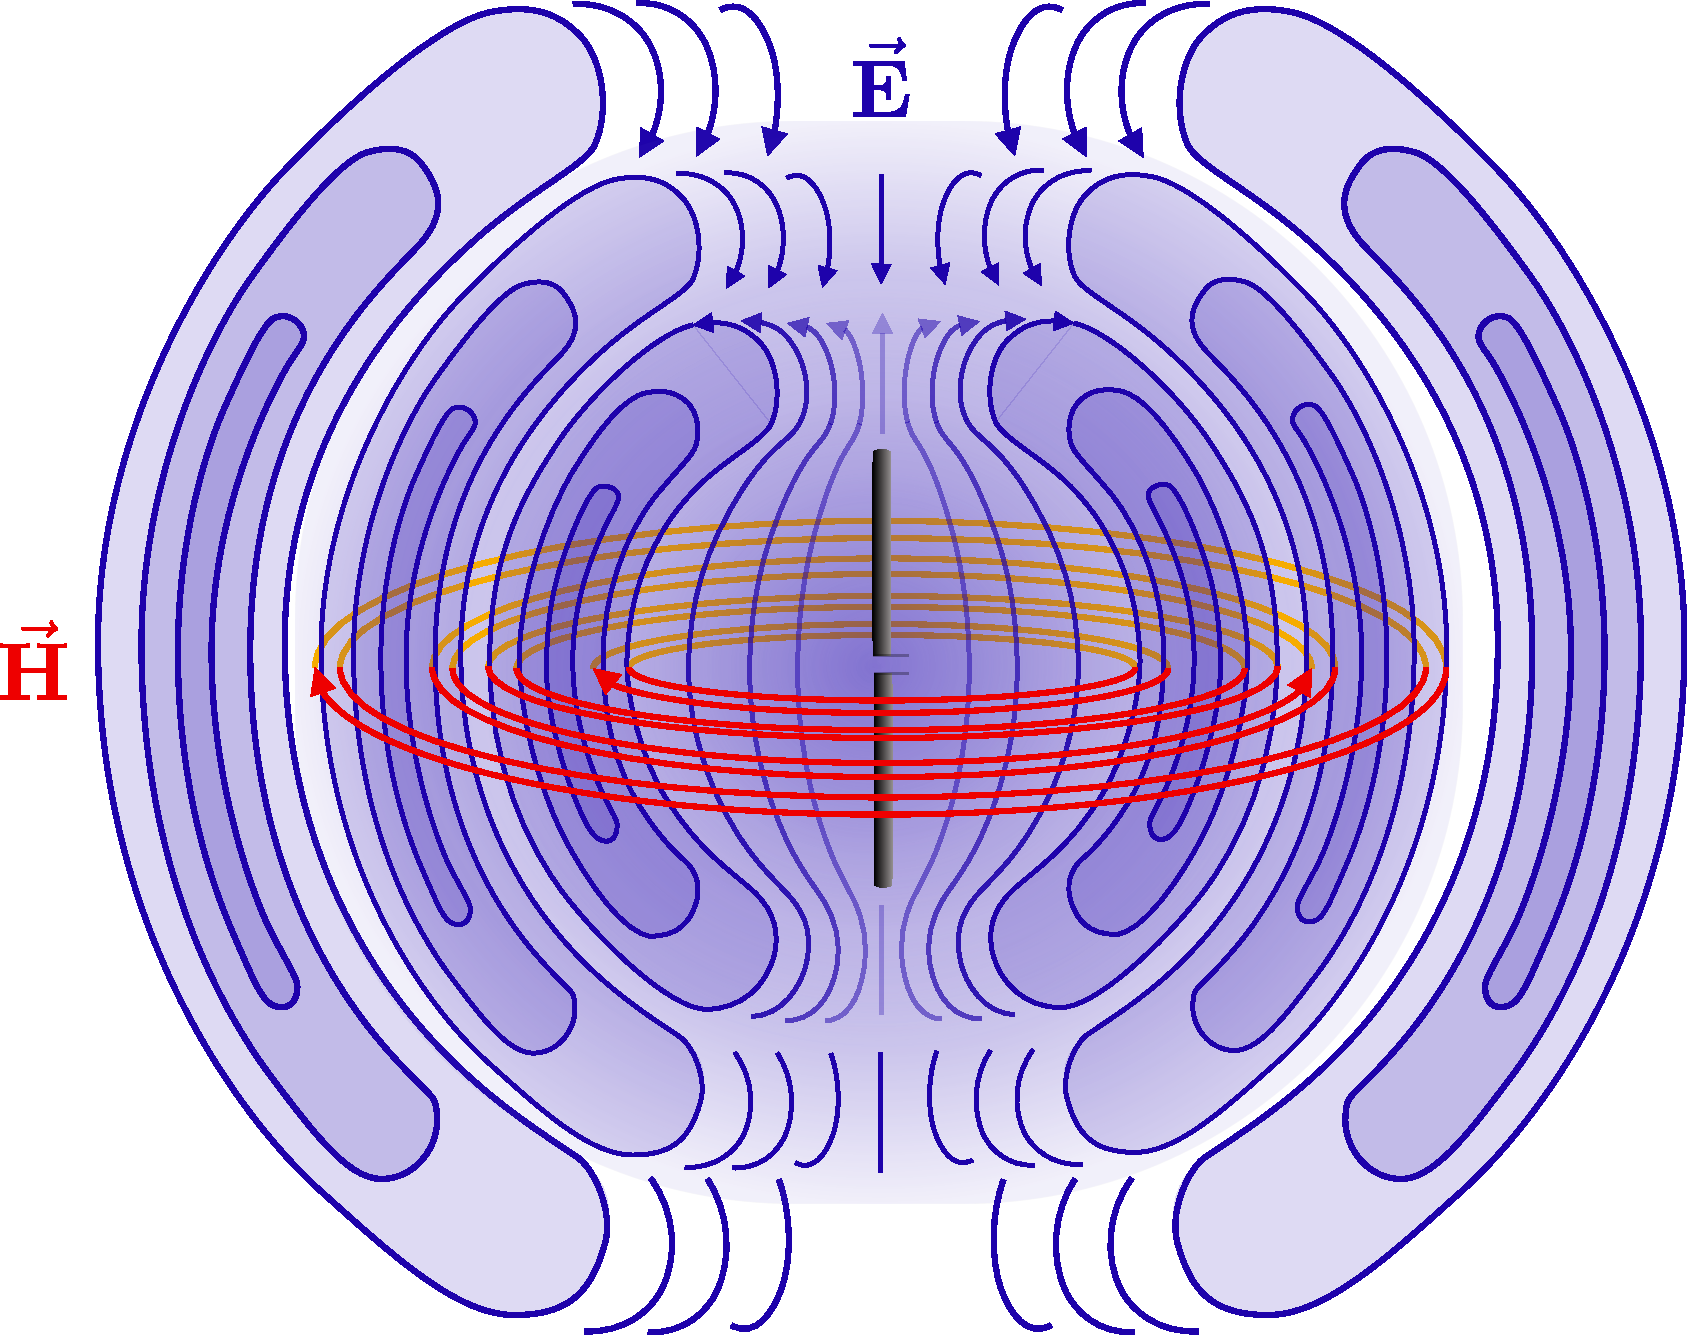
\includegraphics[width=.9\textwidth]{radiation.pdf}
        \caption{Antenna Radiation Mechanism}
      \end{figure}
    \end{column}%
  \end{columns}
\end{frame}

\begin{frame}[fragile]
  \frametitle{Finding the Antenna Fields}
  \begin{outline}
    \1 There are mainly two ways to find the radiated fields from a given current distribution
  \end{outline}
  \begin{figure}
    \centering
    {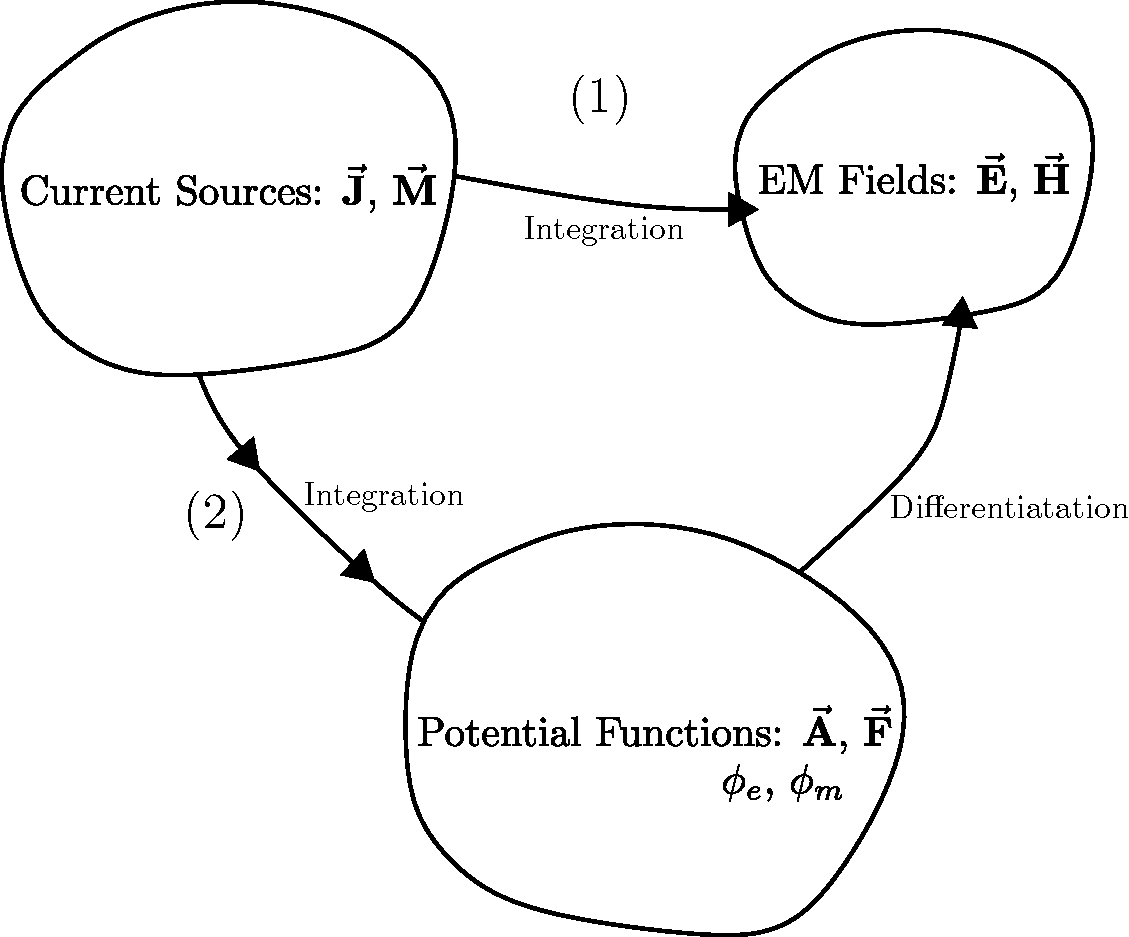
\includegraphics[width=.6\linewidth]{calculation.pdf}
      \label{fig:aug_fields}}
    \caption{Two ways to find the radiated EM fields}
  \end{figure}
\end{frame}


\begin{frame}
  \frametitle{Auxiliary Potential Functions}
  \begin{outline}
    \1 Solving EM fields directly using the Maxwell's equations is often very difficult, especially in the spatial domain
    \1 The introduction of scalar (${\phi}$) and vector $\va{A}$ potential functions simplify the process
    \1 We start from the fact:
    \2 Magnetic field is divergence-less ($\div \va{B} = 0$). We can therefore, say that:
  \end{outline}
  \begin{align*}
    \div \curl \va{A} \equiv 0                       \\
    \Rightarrow \va{H} & = \frac{1}{\u} \curl \va{A}
  \end{align*}
  We can write the Ampere's law as:
  \begin{align*}
    \curl \va{E}                               & = - \j \O \u \va{H} = \j \O \curl \va{A} \\
    \curl \left (\va{E} + \j \O \va{A} \right) & = 0
  \end{align*}
\end{frame}

\begin{frame}
  \frametitle{Auxiliary Potential Functions - contd.}
  Knowing that the $\curl (-\grad \phi) \equiv 0 $, we set:
  \begin{align*}
    \va{E} + \j \O \va{A} & = -\grad \phi                \\
    \va{E}                & = -\grad \phi - \j \O \va{A}
  \end{align*}
  \begin{outline}
    \1 $\phi$ is the electric scalar potential and its a function of position.
    \1 If we know $\va{A}$ and $\phi$, we can find $\va{E}$ and $\va{H}$
  \end{outline}
\end{frame}



\begin{frame}
  \frametitle{How to find the potential functions}

  \begin{outline}
    \1 We still need to figure out how to find the potentials,   $\va{A}$ and $\phi$ for a given current density $\va{J}$.
    \1 For this we move back to Maxwell's equations and find a relationship
  \end{outline}
  \begin{align*}
    \curl \va{H}                      & = \j \O \E \va{E} + \va{J}                                         \\
    \curl \left( \curl \va{A} \right) & = \j \O \u \E \va{E} + \u \va{J}                                   \\
    \curl \curl \va{A}                & = \j \O \u \E \left(-\j \O \va{A} - \grad \phi \right) + \u \va{J}
  \end{align*}
\end{frame}

\begin{frame}
  \frametitle{Finding fields through potential functions}
  Continuing and using the vector identity,
  $\curl \curl \va{A} = \grad ( \div  \va{A} - \laplacian \va{A})$
  and rearranging, we get,
  \begin{align*}
    \laplacian \va{A} + \O^2 \u \E \va{A} & = -\u \va{J} + \grad (\div \va{A} +  \j \O \u \E \phi)
  \end{align*}

  The solution is complete by defining $\va{A}$ in terms of $\phi$ through the Lorentz gauge,
  \begin{align*}
    \div \va{A} & = - \j \O \u \E \phi
  \end{align*}
  The magnetic vector potential $\va{A}$ is finally expressed through an inhomogeneous vector wave equation:
  \begin{align*}
    \laplacian \va{A} + k^2 \va{A} & = -\u \va{J}
  \end{align*}
\end{frame}

\begin{frame}
  \frametitle{Summary - The potential function}
  \begin{outline}
    \1 Given an electric current density $\va{J}$
    \1 Solve for the magnetic vector potential $\va{A}$
    \2 Solve for $\va{E}$ and $\va{H}$
  \end{outline}
  There are some assumptions in this method, namely:
  \begin{outline}
    \1 The space is homogeneous (only one material)
    \1 The magnetic current density $\va{M}$ is zero.
  \end{outline}
\end{frame}


\begin{frame}
  \frametitle{Solving for A given J}
  \begin{outline}
    \1 We solve $\va{A}$ individually in terms of the scalar components ($A_x, A_y, A_z$)
    \1 For a forcing function $p$, the general solution (in terms of $\psi$) can be written as:
  \end{outline}
  \begin{align}
    \laplacian \psi + k^2 \psi & = -p
    \label{eq:scalar_func}
  \end{align}
  For a point source ($p = \delta(\va{r})$), the solution of the above equation is called the \textit{impulse response}. And this impulse response is also called the \color{red}{Green function} of the differential equation
\end{frame}



\begin{frame}
  \frametitle{Solving for A given J}
  \begin{outline}
    \1 For a delta function, the solution of \ref{eq:scalar_func} is 0 everywhere except at the origin.
    \1 Due to spherical symmetry, it is better to express the problem in the spherical coordinates.
  \end{outline}
  \begin{align*}
    \frac{1}{r^2}\pdv{}{r}\left(r^2 \pdv{\psi}{r}\right) & = -k^2 \psi
  \end{align*}
  Substituting $\psi = G/r$, we get:
  \begin{align*}
    \pdv[2]{G}{r} = k^2 G                     \\
    G & = C_1 \e^{-\j k r} + C_2 \e^{+\j k r}
  \end{align*}
  In terms of $\psi$ the solution becomes:
  \begin{align*}
    \psi = \frac{G}{r} & = \frac{C_1}{r} \e^{-\j k r} + \frac{C_2}{r} \e^{+\j k r}
  \end{align*}
  For sources displaced from the origin, we use:
  \begin{align*}
    \va{R} & = \va{r} - \va{r'}
  \end{align*}
\end{frame}

\begin{frame}
  \frametitle{The Hertzian Dipole}
  \begin{outline}
    \1 The fundamental type of antenna is the point electric dipole also known as the \textit{The Hertzian Dipole}
    \1 The current of a z-directed Hertzian dipole is expressed as:
  \end{outline}
  \begin{columns}[T] % align columns
    \begin{column}{.65\textwidth}
      \begin{align*}
        J_z (\va{r}) & = \vu{z} I  \dd{l} \delta(\va{r})
      \end{align*}
      The magnetic vector potential is given as:
      \begin{align*}
        \va{A} & = \vu{z} \u \frac{I}{4 \pi} \dd{l} \frac{\e^{-\j k r}}{r}
      \end{align*}
      For an arbitrary source, we have:
      \begin{align*}
        \va{A} & =   \frac{\u}{4 \pi} \int_{V} \va{J} \dd{v'} \frac{\e^{-\j k r}}{r}
      \end{align*}
    \end{column}
    \begin{column}[T]{.35\textwidth}
      \begin{figure}
        \centering
        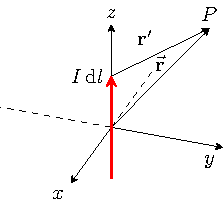
\includegraphics[width=.9\textwidth]{VED_above_half_space.pdf}
        \caption{The Hertzian Dipole}
      \end{figure}
    \end{column}%
  \end{columns}
\end{frame}




\section{Antenna Characteristics and Parameters}


\begin{frame}
  \frametitle{The Radiation Pattern}
  \begin{outline}
    \1 A graphical representation of the \textit{far-field} radiation properties
    \1 Pattern can be further described in \textit{E-} ($E_{\theta}$)and \textit{H-} ($H_{\phi}$) planes.
    \begin{columns}[T] % align columns
      \begin{column}{.35\textwidth}
        For a Hertzian dipole, the far-fields ($k r \gg 1$) are given as:
        \begin{align*}
          \va{E} & = \vu*{\theta} \frac{ \j \O \u I  \dd{l}}{4 \pi r} \sin(\theta) \\
          \va{H} & = \vu*{\phi} \frac{ \j k I  \dd{l}}{4 \pi r} \sin(\theta)
        \end{align*}
      \end{column}
      \begin{column}[T]{.65\textwidth}
        \begin{figure}
          \centering
          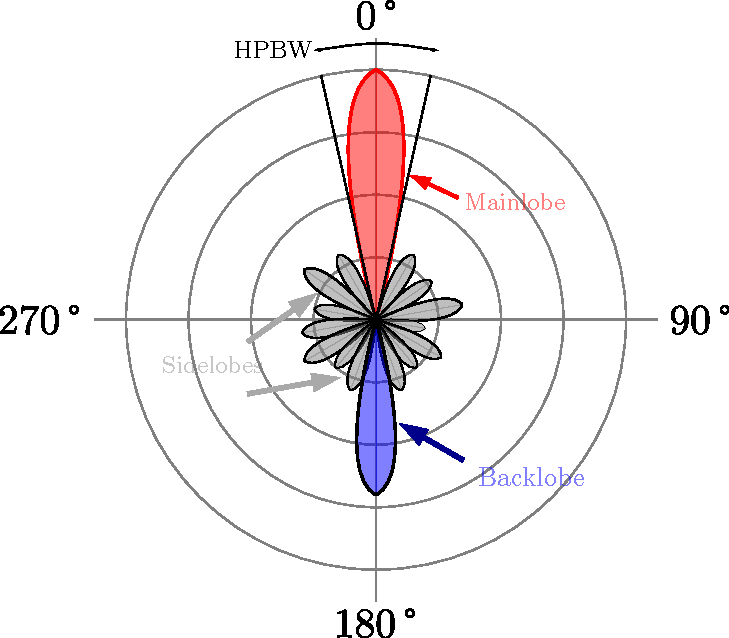
\includegraphics[width=.9\textwidth]{src/lobes.pdf}
          \caption{The Radiation Pattern}
        \end{figure}
      \end{column}%
    \end{columns}
  \end{outline}
\end{frame}

\begin{frame}
  \frametitle{Regions of Radiation}
  \begin{figure}[t!]
    \centering
    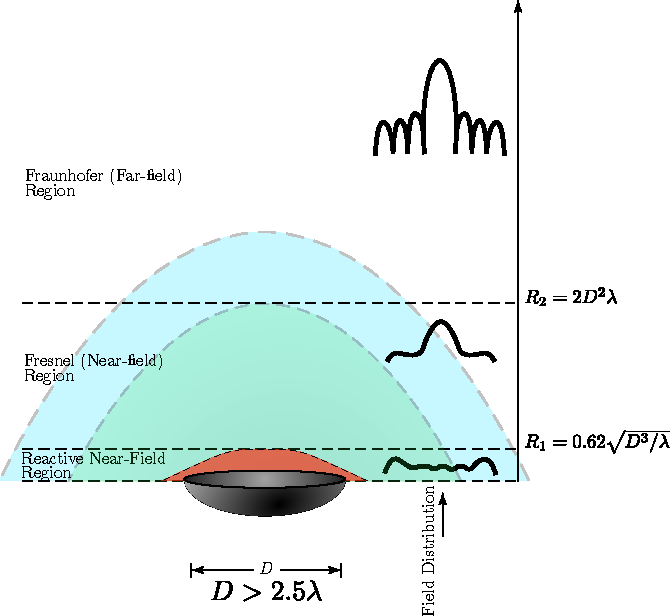
\includegraphics[width=.7\textwidth]{src/antenna_rregions.pdf}
    \caption{The Regions of Antenna Radiation}
  \end{figure}
\end{frame}


\begin{frame}
  \frametitle{Plotting the Radiation Pattern}
  \begin{outline}
    \1 The graphical representation is easier in the spherical coordinates
    \1 We apply the Cartesian to Spherical coordinate transformation
  \end{outline}
  \begin{figure}
    \centering
    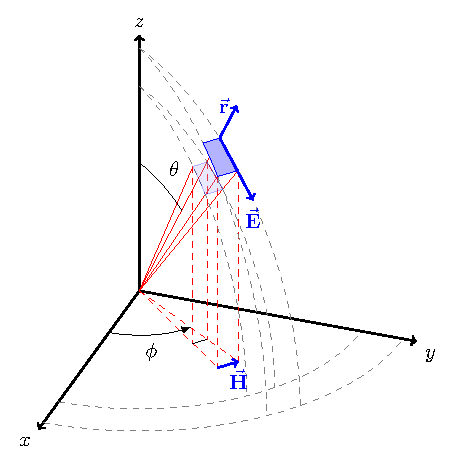
\includegraphics[width=.6\textwidth]{3dcoord.pdf}
  \end{figure}
\end{frame}

\begin{frame}

  \begin{tcolorbox}[colback=blue!5,colframe=university-blue,title=Homework]
    \begin{outline}
      \1 Derive the expressions of the electric and magnetic fields for a loop antenna oriented in the $x-y$ plane as shown below
      \2 First derive the expression of the magnetic vector potential $\va{A}$
      \2 Spherical coordinate transformation needs to be done on the operators and expressions.
      \1 \textcolor{red}{Due on MS Teams on March 30.}
    \end{outline}
  \end{tcolorbox}
  \begin{figure}
    \centering
    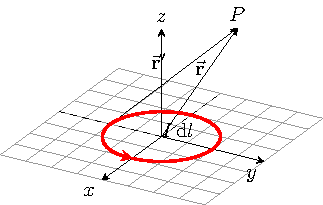
\includegraphics[width=.4\textwidth]{circular.pdf}
  \end{figure}
\end{frame}

\begin{frame}
  \frametitle{Example - The Uniform Line Source}
  \begin{outline}
    \1 A line source with a uniform current along its extent
    \1 Say the line is z-directed and centered on the origin
    \1 The length of the line source is $L$
  \end{outline}
  \begin{align*}
    I (z') & =\left\{\begin{array}{ll}
      I_{0} & x'=0, \quad y=0, \quad |z'| \leq \frac{L}{2} \\
      0     & \text { elsewhere }
    \end{array}\right.
  \end{align*}
  \begin{figure}[t!]
    \centering
    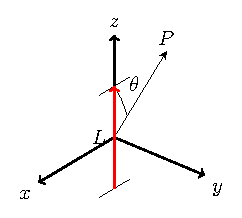
\includegraphics[width=.4\textwidth]{line_source.pdf}
  \end{figure}
\end{frame}

\begin{frame}
  \frametitle{Example - contd.}
  \begin{outline}
    \1 As the current is only in the z-direction, we only find the $A_z$ component
    \1 For z-directed sources, $R \approx r - z' \cos \theta$ for the phase term and $R \approx r$ in the magnitude term
  \end{outline}
  \begin{align*}
    A_z & = \u \int_{-L/2}^{L/2} I(z') \frac{\e^{-\j k R}}{4 \pi R} \dd{z'}                                     \\
        & = \u \frac{\e^{-\j k r}}{4 \pi r} \int_{-L/2}^{L/2} I_0 \e^{\j k \left(z' \cos \theta\right)} \dd{z'} \\
        & = \u \frac{I_0 \e^{-\j k r}}{4 \pi r} \frac{\sin \left[(kL/2)\cos \theta\right]}{(kL/2)\cos \theta}
  \end{align*}
\end{frame}

\begin{frame}
  \frametitle{Example - contd.}
  The electric field is given as:
  \begin{align*}
    \va{E} & = - \j \O \va{A} - \frac{\j}{\O \u \E} \grad(\div \va{A})                                                                                      \\
           & = - \j \O \va{A} - (- \j \O \va{A} \cdot \vu{r})\vu{r}                                                                                         \\
           & = \j \O \sin \theta A_z \vu*{\theta}                                                                                                           \\
           & = \frac{\j \O \u I_{0} L \e^{-\j k r}}{4 \pi r} \sin \theta \frac{\sin \left[(k L / 2) \cos \theta\right]}{(k L / 2) \cos \theta} \vu*{\theta}
  \end{align*}
  The magnetic field can simply be found as:
  \begin{align*}
    H_{\phi} & = \frac{E_{\theta}}{\eta}
  \end{align*}
\end{frame}

\begin{frame}
  \frametitle{The Poynting Vector}
  \begin{outline}
    \1 This describes the \textit{complex power density} flowing out of a sphere of radius $r$
    \1 It is real-valued and directed along the wave propagation direction
  \end{outline}
  \begin{align*}
    \va{S} & = \frac{1}{2} \va{E} \cross \va{H^{*}}
  \end{align*}
  \begin{outline}
    \1 If $\va{E}$ is in the $\vu*{\theta}$ and $\va{H}$ is in the $\vu*{\phi}$ directions
    \1 The Poynting vector will be radially directed.
  \end{outline}
\end{frame}


\begin{frame}
  \frametitle{The Intrinsic Impedance}
  \begin{outline}
    \1 Just like voltage and current ratio gives us impedance
    \1 The ratio of electric and magnetic field components give us the \textit{intrinsic impedance}
  \end{outline}
  \begin{align*}
    \frac{E_{\theta}}{H_{\phi}} & = \eta = \sqrt{\frac{\u}{\E}}
  \end{align*}
  For freespace, the value is $\eta_0 = \SI{376.7}{\ohm} \approx \SI{120 \pi}{\ohm}$
\end{frame}


\begin{frame}
  \frametitle{Antenna Power}
  \begin{outline}
    \1 The total power radiated by an antenna can be found from the Poynting vector
    \1 We need to integrate over a surface
  \end{outline}
  \begin{align*}
    P & = \iint_{S'} \va{S} \cdot \dd{S'} = 1/2 \Re \iint_{S'} \left( \va{E} \cross \va{H^{*}}\right) \cdot \dd{S'}
  \end{align*}
  The $\dd{S'}$ in spherical coordinates refers to a solid angle and for a given radius $r$ can be expressed as:
  \begin{align*}
    \dd{S'} & = r^2 \sin \theta \dd{\theta} \dd{\phi}
  \end{align*}
\end{frame}

\begin{frame}
  \frametitle{Radiation Intensity}
  \begin{outline}
    \1 Since the power varies with distance $r$, it is convenient to define the \textit{radiation intensity}
    \1 The radiation intensity is independent of the distance
    \1 It is defined as the \color{red}{power radiated in a given direction per unit solid angle}
    \2 It has units of watts per steradians
  \end{outline}
  \begin{align*}
    U(\theta, \phi) & = \frac{1}{2} \Re \left(\va{E} \cross \va{H^{*}}\right) \cdot r^2 \vu{r}
  \end{align*}
\end{frame}

\begin{frame}
  \frametitle{Directivity and Gain}
  \begin{outline}
    \1 For a given antenna the directivity and gain describe in what direction the radiation is, as compared to an isotropic antenna
    \1 For the isotropic antenna, the radiation pattern is uniform (ie) a circle
    \1 Directivity is defined as the ratio of radiation intensity in a certain direction to the average radiation intensity
  \end{outline}
  \begin{align*}
    D & = \frac{1}{2} \frac{\max \left[\Re (\va{E} \cross \va{H^{*}}) \cdot \vu{r} \right]}{P /4 \pi r^2}
  \end{align*}
\end{frame}

\begin{frame}
  \frametitle{Visualising the Directivity}
  \begin{figure}
    \centering
    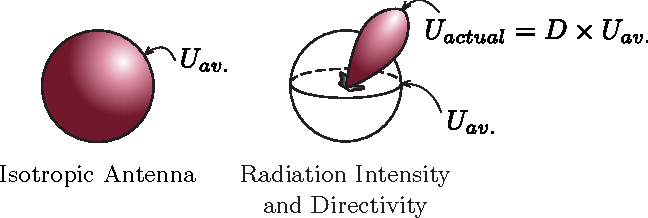
\includegraphics[width=.8\textwidth]{src/antenna_dir.pdf}
    \caption{Relationship between Radiation Intensity and Directivity}
  \end{figure}
\end{frame}


\begin{frame}
  \frametitle{Antenna Gain}
  \begin{outline}
    \1 Although the directivity describes the radiation pattern of an antenna, we need a quantity that can be used when treating antenna as a system
    \1 Suppose the antenna is one component of a radio-frequency system that includes transmission lines and sources
    \1 A parameter is helpful that determines how \textit{efficiently} the antenna operates
    \2 In particular, how much input power is transferred into radiated power
    \1 Antenna gain is defined as:
  \end{outline}
  \begin{align*}
    G & = 4 \pi \frac{U_m}{P_m}
  \end{align*}
  We often describe it in terms of decibels:
  \begin{align*}
    G_{\mathrm{dB}} & = 10 \log G
  \end{align*}
\end{frame}

\begin{frame}
  \frametitle{Radiation Impedance}
  \begin{outline}
    \1 We can treat antenna as an impedance with real and imaginary parts
    \2 The real part refers to the how much radiation leaves the antenna $(R_r)$ and how much dissipates as losses $(R_o)$
    \2 The imaginary part $(X_A)$ determines the stored power in the near field.
  \end{outline}
  \begin{align*}
    Z_A & = R_A + \j X_A = (R_r + R_{ohm}) + \j X_A
  \end{align*}
\end{frame}

\begin{frame}
  \frametitle{Radiation Efficiency}
  \begin{outline}
    \1 Efficiency is a metric that determines the ratio of total desired power to the total power supplied
    \1 Radiation efficiency of antennas is a measure how much power is radiated
  \end{outline}
  \begin{align*}
    e_{rad} & = \frac{P_{rad}}{P_{in}} = \frac{P_{rad}}{P_{rad} + P_{ohm}}
  \end{align*}
\end{frame}


\end{document}
